\de{ĐỀ THI GIỮA HỌC KỲ I NĂM HỌC 2023-2024}{THPT Trần Hưng Đạo}
\begin{bt}%%[1D1H3-3]%[Dự án đề kiểm tra Toán 11 GHKI NH23-24- Lê Minh Thiện Anh]%[THPT - Tp HCM]
	Cho $\sin x=\dfrac{1}{3}$ với $90^{\circ}<x<180^{\circ}$. Tính $\cos x$, $\sin 2x$ và $\cos \left(x-30^{\circ}\right)$.
	\loigiai{
		Ta có 
		\begin{eqnarray*}
		& & \sin^2x+\cos^2x=1\\
		&\Leftrightarrow & \left(\dfrac{1}{3}\right)^2+\cos^2x=1\\
		&\Leftrightarrow & \cos^2x=\dfrac{8}{9}\\
		&\Leftrightarrow & \cos x=\pm \dfrac{2\sqrt{2}}{3}.
		\end{eqnarray*}
		Vì $90^{\circ}<x<180^{\circ}$ nên $\cos x=-\dfrac{2\sqrt{2}}{3}$.\\
		Khi đó $\sin 2x=2\sin x\cos x=2\cdot \dfrac{1}{3}\cdot \left( -\dfrac{2\sqrt{2}}{3}\right)=-\dfrac{4\sqrt{2}}{9}$.\\
		$\cos \left(x-30^{\circ}\right)=\cos x\cos 30^\circ+\sin x\sin 30^\circ=-\dfrac{2\sqrt{2}}{3}\cdot\dfrac{\sqrt{3}}{2}+\dfrac{1}{3}\cdot \dfrac{1}{2}=\dfrac{1-2\sqrt{6}}{6}$.
	}
\end{bt}

\begin{bt}%[1D1H4-2]%[Dự án đề kiểm tra Toán 11 GHKI NH23-24- Lê Minh Thiện Anh]%[THPT - Tp HCM]
	Tìm tập xác định của hàm số $y=-3 \cot \left(x-\dfrac{\pi}{3}\right)+1$.
	\loigiai{
		Hàm số đã cho xác định khi 
		\begin{eqnarray*}
		& & \sin \left(x-\dfrac{\pi}{3}\right)\neq 0\\
		&\Leftrightarrow & x-\dfrac{\pi}{3}\neq k\pi\\
		&\Leftrightarrow & x\neq \dfrac{\pi}{3}+k\pi \,(k\in \mathbb{Z}).
		\end{eqnarray*}
		Vậy tập xác định của hàm số đã cho là $\mathscr{D}=\mathbb{R} \setminus \left\lbrace \dfrac{\pi}{3}+k\pi,k\in\mathbb{Z}\right\rbrace$.
	}
\end{bt}

\begin{bt}%[1D1H5-5]%[Dự án đề kiểm tra Toán 11 GHKI NH23-24- Lê Minh Thiện Anh]%[THPT - Tp HCM]
	Giải phương trình $\cos x-\sin \left(2x-\dfrac{\pi}{3}\right)=0$.
	\loigiai{
		Ta có
		\begin{eqnarray*}
		& & \cos x-\sin \left(2x-\dfrac{\pi}{3}\right)=0\\
		&\Leftrightarrow & \cos x=\sin \left(2x-\dfrac{\pi}{3}\right)\\
		&\Leftrightarrow & \cos x=\cos \left(\dfrac{5\pi}{6}-2x\right)\\
		&\Leftrightarrow & \hoac{& x= \dfrac{5\pi}{6}-2x+k2\pi \\& x= 2x-\dfrac{5\pi}{6}+k2\pi}\\
		&\Leftrightarrow & \hoac{& x=\dfrac{5\pi}{18}+\dfrac{k2\pi}{3} \\& x=\dfrac{5\pi}{6}+k2\pi} (k\in \mathbb{Z}).
		\end{eqnarray*}
		Vậy phương trình có tập nghiệm $S=\left\lbrace\dfrac{5\pi}{18}+\dfrac{k2\pi}{3},\dfrac{5\pi}{6}+k2\pi, k\in \mathbb{Z} \right\rbrace$.
	}
\end{bt}
\begin{bt}%[1D1V4-7]%[1D1V4-8]%[Dự án đề kiểm tra Toán 11 GHKI NH23-24- Thinh Ngo]%[THPT Trần Hưng Đạo]
	Nhiệt độ ngoài trời ở một thành phố vào các thời điểm khác nhau trong ngày có thể được mô phỏng bởi công thức $f(t)=29 + 8\cos\left[\dfrac{\pi}{4}\left( 4-\dfrac{t}{3}\right) \right]$, với $f$ tính bằng độ C và $t$ tính bằng giờ ($0\leq t \leq 24$).
	\begin{enumerate}
		\item Nhiệt độ cao nhất trong ngày là bao nhiêu độ C và vào lúc mấy giờ?
		\item Các công nhân công ty môi trường muốn cắt tỉa các cây trồng ở dải phân cách hai làn đường, họ bắt đầu làm việc từ $6$ giờ và kết thúc lúc $17$ giờ trong ngày. Dựa vào đồ thị hàm số côsin (xem hình bên dưới), hãy cho biết họ nên làm việc vào những thời điểm nào trong ngày để tránh nhiệt độ trên $36^\circ$C (kết quả làm tròn đến hàng phần mười).
		\begin{center}
			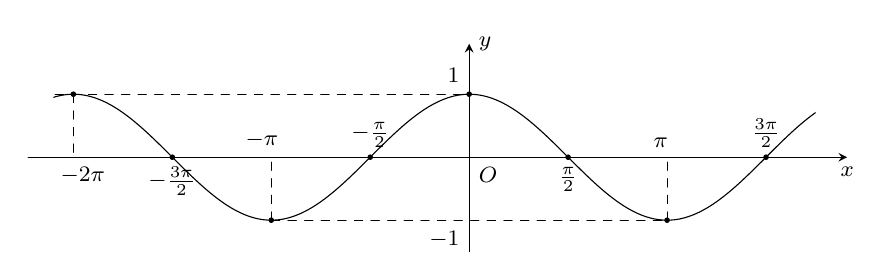
\begin{tikzpicture}[scale=0.8,>=stealth, font=\footnotesize, line join=round, line cap=round]
				\def\xmin{-10} \def\xmax{10.5} \def\ymin{-1.5} \def\ymax{1.8}
				\draw[->] (-7,0)--(6,0) node [below]{$x$};
				\draw[->] (0,\ymin)--(0,\ymax) node [right]{$y$};
				\node at (0,0) [below right]{$O$};
				\clip (\xmin+3.4,\ymin+0.1) rectangle (\xmax-5,\ymax-0.1);
				\draw[smooth,samples=400,domain=\xmin:\xmax] plot(\x,{cos(\x r)});
				\draw[dashed] (\xmin,1)--(0,1) (-3.14,-1)--(3.14,-1);		
				\foreach \x in {-2*pi,-1.5*pi,-pi,-0.5*pi,0}
				{\draw[fill=black] (\x,cos \x*180/pi) circle (1pt);
					\draw[dashed] (\x,cos \x*180/pi)--(\x,0);
					\draw[fill=black] (-\x,cos -\x*180/pi) circle (1pt);
					\draw[dashed] (-\x,cos \x*180/pi)--(-\x,0);}
				\node at (0,1.3) [left]{$1$};
				\node at (0,-1.3) [left]{$-1$};
				\node at (-2*pi+0.15,0) [below]{$-2\pi$};
				\node at (-1.5*pi,0) [below]{$-\frac{3\pi}{2}$};
				\node at (-pi-0.15,0) [above]{$-\pi$};
				\node at (-0.5*pi,0) [above]{$-\frac{\pi}{2}$};
				\node at (0.5*pi,0) [below]{$\frac{\pi}{2}$};
				\node at (pi-0.1,0) [above]{$\pi$};
				\node at (1.5*pi,0) [above]{$\frac{3\pi}{2}$};
			\end{tikzpicture}
		\end{center}
	\end{enumerate} 
	
	\loigiai{
	\begin{enumerate}
		\item Ta có
		\begin{eqnarray*} 
		&-1&\leq \cos\left[\dfrac{\pi}{4}\left( 4-\dfrac{t}{3}\right) \right]\leq 1\\ &\Leftrightarrow& - 8 \leq  8\cos\left[\dfrac{\pi}{4}\left( 4-\dfrac{t}{3}\right) \right]\leq 8\\ &\Leftrightarrow& 21 \leq 29 + 8\cos\left[\dfrac{\pi}{4}\left( 4-\dfrac{t}{3}\right) \right] \leq 37\\
		&\Leftrightarrow& 21 \leq f(t)\leq 37.
		\end{eqnarray*}
	$\text{Max} f(t) = 37$ khi $\cos\left[\dfrac{\pi}{4}\left( 4-\dfrac{t}{3}\right) \right] = 1\Leftrightarrow \dfrac{\pi}{4}\left( 4-\dfrac{t}{3}\right) = k2\pi \Leftrightarrow t = 3(4-8k)$.\\
	Do $0\leq t \leq 24$ cho nên $-\dfrac{1}{2}\leq k \leq \dfrac{1}{2}$ ta chọn $k = 0 \Rightarrow t = 12$.\\ 
	Vậy nhiệt độ cao nhất trong ngày là $37$ độ C vào lúc $12$ giờ.
	\item 
	\begin{center}
		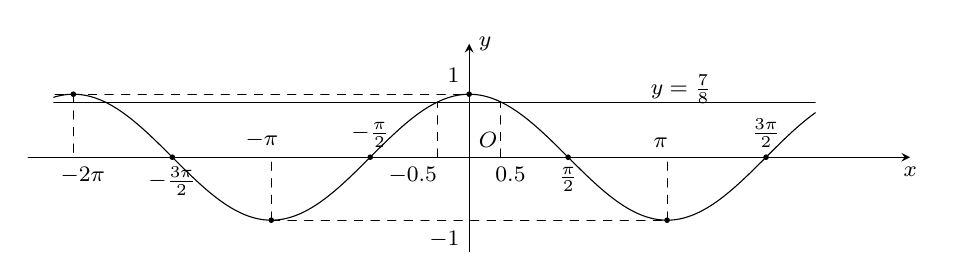
\begin{tikzpicture}[scale=0.8,>=stealth, font=\footnotesize, line join=round, line cap=round]
			\def\xmin{-10} \def\xmax{10.5} \def\ymin{-1.5} \def\ymax{1.8}
			\draw[->] (-7,0)--(7,0) node [below]{$x$};
			\draw[->] (0,\ymin)--(0,\ymax) node [right]{$y$};
			\node at (0,0) [above right]{$O$};
			\clip (\xmin+3.4,\ymin+0.1) rectangle (\xmax-5,\ymax-0.1);
			\draw[smooth,samples=400,domain=\xmin:\xmax] plot(\x,{cos(\x r)});
			\draw[dashed] (\xmin,1)--(0,1) (-3.14,-1)--(3.14,-1);
			\draw
			(\xmin,7/8)--(\xmax,7/8);
			\foreach \x in {-2*pi,-1.5*pi,-pi,-0.5*pi,0}
			{\draw[fill=black] (\x,cos \x*180/pi) circle (1pt);
				\draw[dashed] (\x,cos \x*180/pi)--(\x,0);
				\draw[fill=black] (-\x,cos -\x*180/pi) circle (1pt);
				\draw[dashed] (-\x,cos \x*180/pi)--(-\x,0);}
			\node at (0,1.3) [left]{$1$};
			\node at (0,-1.3) [left]{$-1$};
			\node at (-2*pi+0.15,0) [below]{$-2\pi$};
			\node at (0.161*pi+0.15,0) [below  ]{$0.5$};
			\node at (-0.161*pi+0.15,0) [below left ]{$-0.5$};
			\node at (4.0,0.7) [above left ]{$y = \frac{7}{8}$};
			\node at (-1.5*pi,0) [below]{$-\frac{3\pi}{2}$};
			\node at (-pi-0.15,0) [above]{$-\pi$};
			\node at (-0.5*pi,0) [above]{$-\frac{\pi}{2}$};
			\node at (0.5*pi,0) [below]{$\frac{\pi}{2}$};
			\node at (pi-0.1,0) [above]{$\pi$};
			\node at (1.5*pi,0) [above]{$\frac{3\pi}{2}$};
			\draw[dashed] (0.5,0)--(0.5,7/8);
			\draw[dashed] (-0.5,0)--(-0.5,7/8);
		\end{tikzpicture}
	\end{center}
	Theo đề bài ta có
	\begin{eqnarray*} 
	 &f(t)& \leq 36 \\&\Leftrightarrow& 29 + 8\cos\left[\dfrac{\pi}{4}\left( 4-\dfrac{t}{3}\right) \right] \leq 36\\ &\Leftrightarrow & \cos\left[\dfrac{\pi}{4}\left( 4-\dfrac{t}{3}\right) \right] \leq \dfrac{7}{8}\\& \Leftrightarrow& -0{,}5  \leq \dfrac{\pi}{4}\left( 4-\dfrac{t}{3}\right) \leq 0{,}5\\& \Leftrightarrow& 10{,}1 \leq t \leq 13{,}9.
	 \end{eqnarray*}
	\end{enumerate}

	Như vậy để tránh nhiệt độ trên $36^\circ$C thì các công nhân làm việc từ $10{,1}$ giờ đến $13{,}9$ giờ.
	}
\end{bt}


\begin{bt}%[1D2H2-4]%[Dự án đề kiểm tra Toán 11 GHKI NH23-24- Thinh Ngo]%[THPT Trần Hưng Đạo]
	Cho cấp số cộng $\left(u_n\right)$ thỏa mãn $\heva{& u_1 + u_6 = 18 \\ & u_3 + u_7 = 22}$. Tìm $u_{20}$. 
	
	\loigiai{$\heva{& u_1 + u_6 = 18 \\ & u_3 + u_7 = 22} \Leftrightarrow \heva{& u_1 + u_1+5d = 18 \\ & u_1+2d + u_1+6d = 22}\Leftrightarrow \heva{& 2u_1 + 5d = 18 \\ & 2u_1+8d = 22} \Leftrightarrow \heva{& u_1 = \dfrac{17}{3} \\ & d = \dfrac{4}{3}.}$\\
	Như vậy $u_{20}=u_1+19d=\dfrac{17}{3}+19 \cdot \dfrac{4}{3} = 31$.	
	}
\end{bt}
%=======================================
\begin{bt}%[1D2V2-7]%[Dự án đề kiểm tra Toán 11 GHKI NH23-24- Nguyễn Đức Lợi]%[THPT Trần Hưng Đạo]
	Anh Hải muốn tiết kiệm tiền để mua một đôi giày chơi bóng rổ giá $3\,840\,000$ đồng. Do đó, anh Hải quyết định bắt đầu mỗi ngày tiết kiệm với ngày đầu $5\,000$ đồng, ngày sau cao hơn ngày trước $2\,000$ đồng. Hỏi anh Hải phải tiết kiệm bao nhiêu ngày thì đủ tiền mua đôi giày đó.
	\loigiai{
	Số tiền tiết kiệm ở ngày thứ nhất là: $u_1 = 5\,000$ (đồng).\\ 
	Vì số tiền tiết kiệm ở ngày sau cao hơn ngày trước $2\,000$ nên số tiền tiết kiệm ở mỗi ngày của anh Hải là một cấp số cộng có $u_1 = 5\,000$ và công bội $d = 2\,000$ (đồng).\\ 
	Sau $n$ ngày, tổng số tiền anh Hải tiết kiệm được là
	$$S_n = \dfrac{n[2u_1  + (n-1)d]}{2} = \dfrac{n[10\,000  + 2\,000(n-1)]}{2} = \dfrac{n( 2\,000 n + 8\,000)}{2}.$$
	Để đủ tiền mua đôi giày đó thì 
	\begin{eqnarray*}
	 S_n \ge 3\,840\,000 & \Leftrightarrow & \dfrac{n( 2\,000 n + 8\,000)}{2} \ge 3\,840\,000\\
	 & \Leftrightarrow & n(n+4) \ge 3\,840 \Leftrightarrow n^2 + 4n - 3\,840 \ge 0\\
	 & \Leftrightarrow & \hoac{& n \le -64 \\ & n \ge 60.}
	\end{eqnarray*}
	Vậy anh Hải phải tiết kiệm ít nhất $60$ ngày mới đủ tiền mua đôi giày đó.
	}
\end{bt}
%=======================================
\begin{bt}%[1H4H1-3]%[1H4H1-4]%[1H4V1-6]%[Dự án đề kiểm tra Toán 11 GHKI NH23-24- Thinh Ngo]%[THPT Trần Hưng Đạo]
	Cho hình chóp $S.ABCD$ có đáy $ABCD$ là tứ giác có các cặp cạnh đối không song song. Gọi $M$ là trung điểm của $SD$.
	\begin{enumerate}
		\item Tìm giao tuyến của hai mặt phẳng $(SAD)$ và $(SBC)$.
		\item Tìm giao điểm $I$ của $BM$ và mặt phẳng $(SAC)$.
		\item Gọi $N$ là giao điểm của $AI$ và $SC$. Chứng minh ba đường thẳng $AB$, $CD$, $MN$ đồng quy.
	\end{enumerate}
	\loigiai{
	\begin{center}
   	\begin{tikzpicture}[thick,font=\scriptsize,scale=1]
	\def\a{4}
	\path 	(0:0) coordinate (A)
			++(0:0.8*\a) coordinate (D)
			++(-110:0.4*\a) coordinate (C)
			($(A)+(-90:0.6*\a)$) coordinate (B)
			($(A)+(60:0.7*\a)$) coordinate (S)
			($(S)!0.5!(D)$) coordinate (M)
			(intersection of A--D and B--C) coordinate (E)
			(intersection of A--C and B--D) coordinate (O)
			(intersection of S--O and B--M) coordinate (I)
			(intersection of A--I and S--C) coordinate (N)
			;
	\draw[thick] (S)--(A)--(B)--(C) (E)--(S)--(C)--(E) (S)--(B)--(N);
	\draw[dashed,thick](M)--(A)--(E) (S)--(D)--(C) (B)--(M)--(N) (A)--(C) (B)--(D) (S)--(O) (A)--(N);
	\foreach \x/\g in {A/-180,B/-135,C/-60,D/60,S/90,M/45,E/0,O/-90,I/150,N/10}
			\fill[black] 	(\x) circle (1pt)
			($(\g:3mm)+(\x)$) node {$\x$};	
	\end{tikzpicture}
   	\end{center}
   	\begin{enumerate}
   		\item Trong mặt phẳng $(ABCD)$, gọi $E = AD \cap BC$.\\
   		Suy ra $(SAD) \cap (SAC) = SE$.
   		\item Trong mặt phẳng $(ABCD)$, gọi $O = AC \cap BD$.\\
   		Trong mặt phẳng $(SBD)$, gọi $I = SO \cap BM$.\\
   		Suy ra $I = BM \cap (SAC)$.
   		\item Trong mặt phẳng $(SAC)$, gọi $N = AI \cap SC$.\\
   		Xét ba mặt phẳng $(ABNM)$, $((ABCD)$, $(SCD)$ có $\heva{& (ABNM)\cap (ABCD) = AB \\& (ABNM) \cap (SCD) = NM\\ & (ABCD)\cap (SCD) = CD.}$\\
   		 Suy ra $AB$, $NM$, $CD$ hoặc đôi một song song hoặc đồng quy tại một điểm.\\
   		Mặt khác $AB$ và $CD$ không song song với nhau, do đó $AB$, $NM$, $CD$ đồng quy tại một điểm.
   		
   	\end{enumerate}
	}
\end{bt}
